\documentclass[../thesis/thesis.tex]{subfiles}
\begin{document}
 \chapter{Methods}

 \section{Classifier Experiment Set 1 Setup}
The first experiment performed with the prototype described in the previous chapter was set out as indicated in \Fref{fig:exps:3setup}. This experiment involved 3 people, who entered the scene in either standing or sitting positions. The following scripts were observed;

\begin{enumerate}
\item One person walks in, stands in center, walks out of frame
\item One person walks in, joined by another person, both stand there, one leaves, then another leaves
\item One person walks in, joined by 1, joined by another, all stand there, one leaves, then another, then another
\item Two people walk in, both stand there, both leave
\item (sitting) One person walks in, sits in center,  moves to right, walks out of frame
\item (sitting) One person walks in, joined by another person, both sit there, switch chairs, one leaves, then another leaves
\item (sitting) One person walks in, joined by 1, joined by another, all sit there, one leaves, then another, then another
\item (sitting) Two people walk in, both sit there, both leave
\end{enumerate}

These experiments were recorded with a thermal-visual synchronization at 1Hz over approximately 60 second intervals each. Each experiment had 10-15 seconds at the beginning where nothing was within the view of the sensor to allow the thermal background to be calculated. Each frame generated from these experiments was manually tagged with the ground truth value of its occupancy using the script mentioned previously. The resulting features and ground truth were exported to a format allowing the Weka machine learning program to analyze them. This data was analyzed with the feature vectors always being considered numeric data and with the ground truth considered both numeric and nominal (categories {0,1,2,3}). The machine learning algorithms J48, Multilayer Perceptron, KStar, IBk, Naive Bayes and SMO were used for the nominal representation, and the algorithms Linear Regression, Multilayer Perceptron and IBk were used for the numeric representation.


\begin{landscape}
 \begin{figure}
 \centering
 % TODO: Proper merging of these figures
 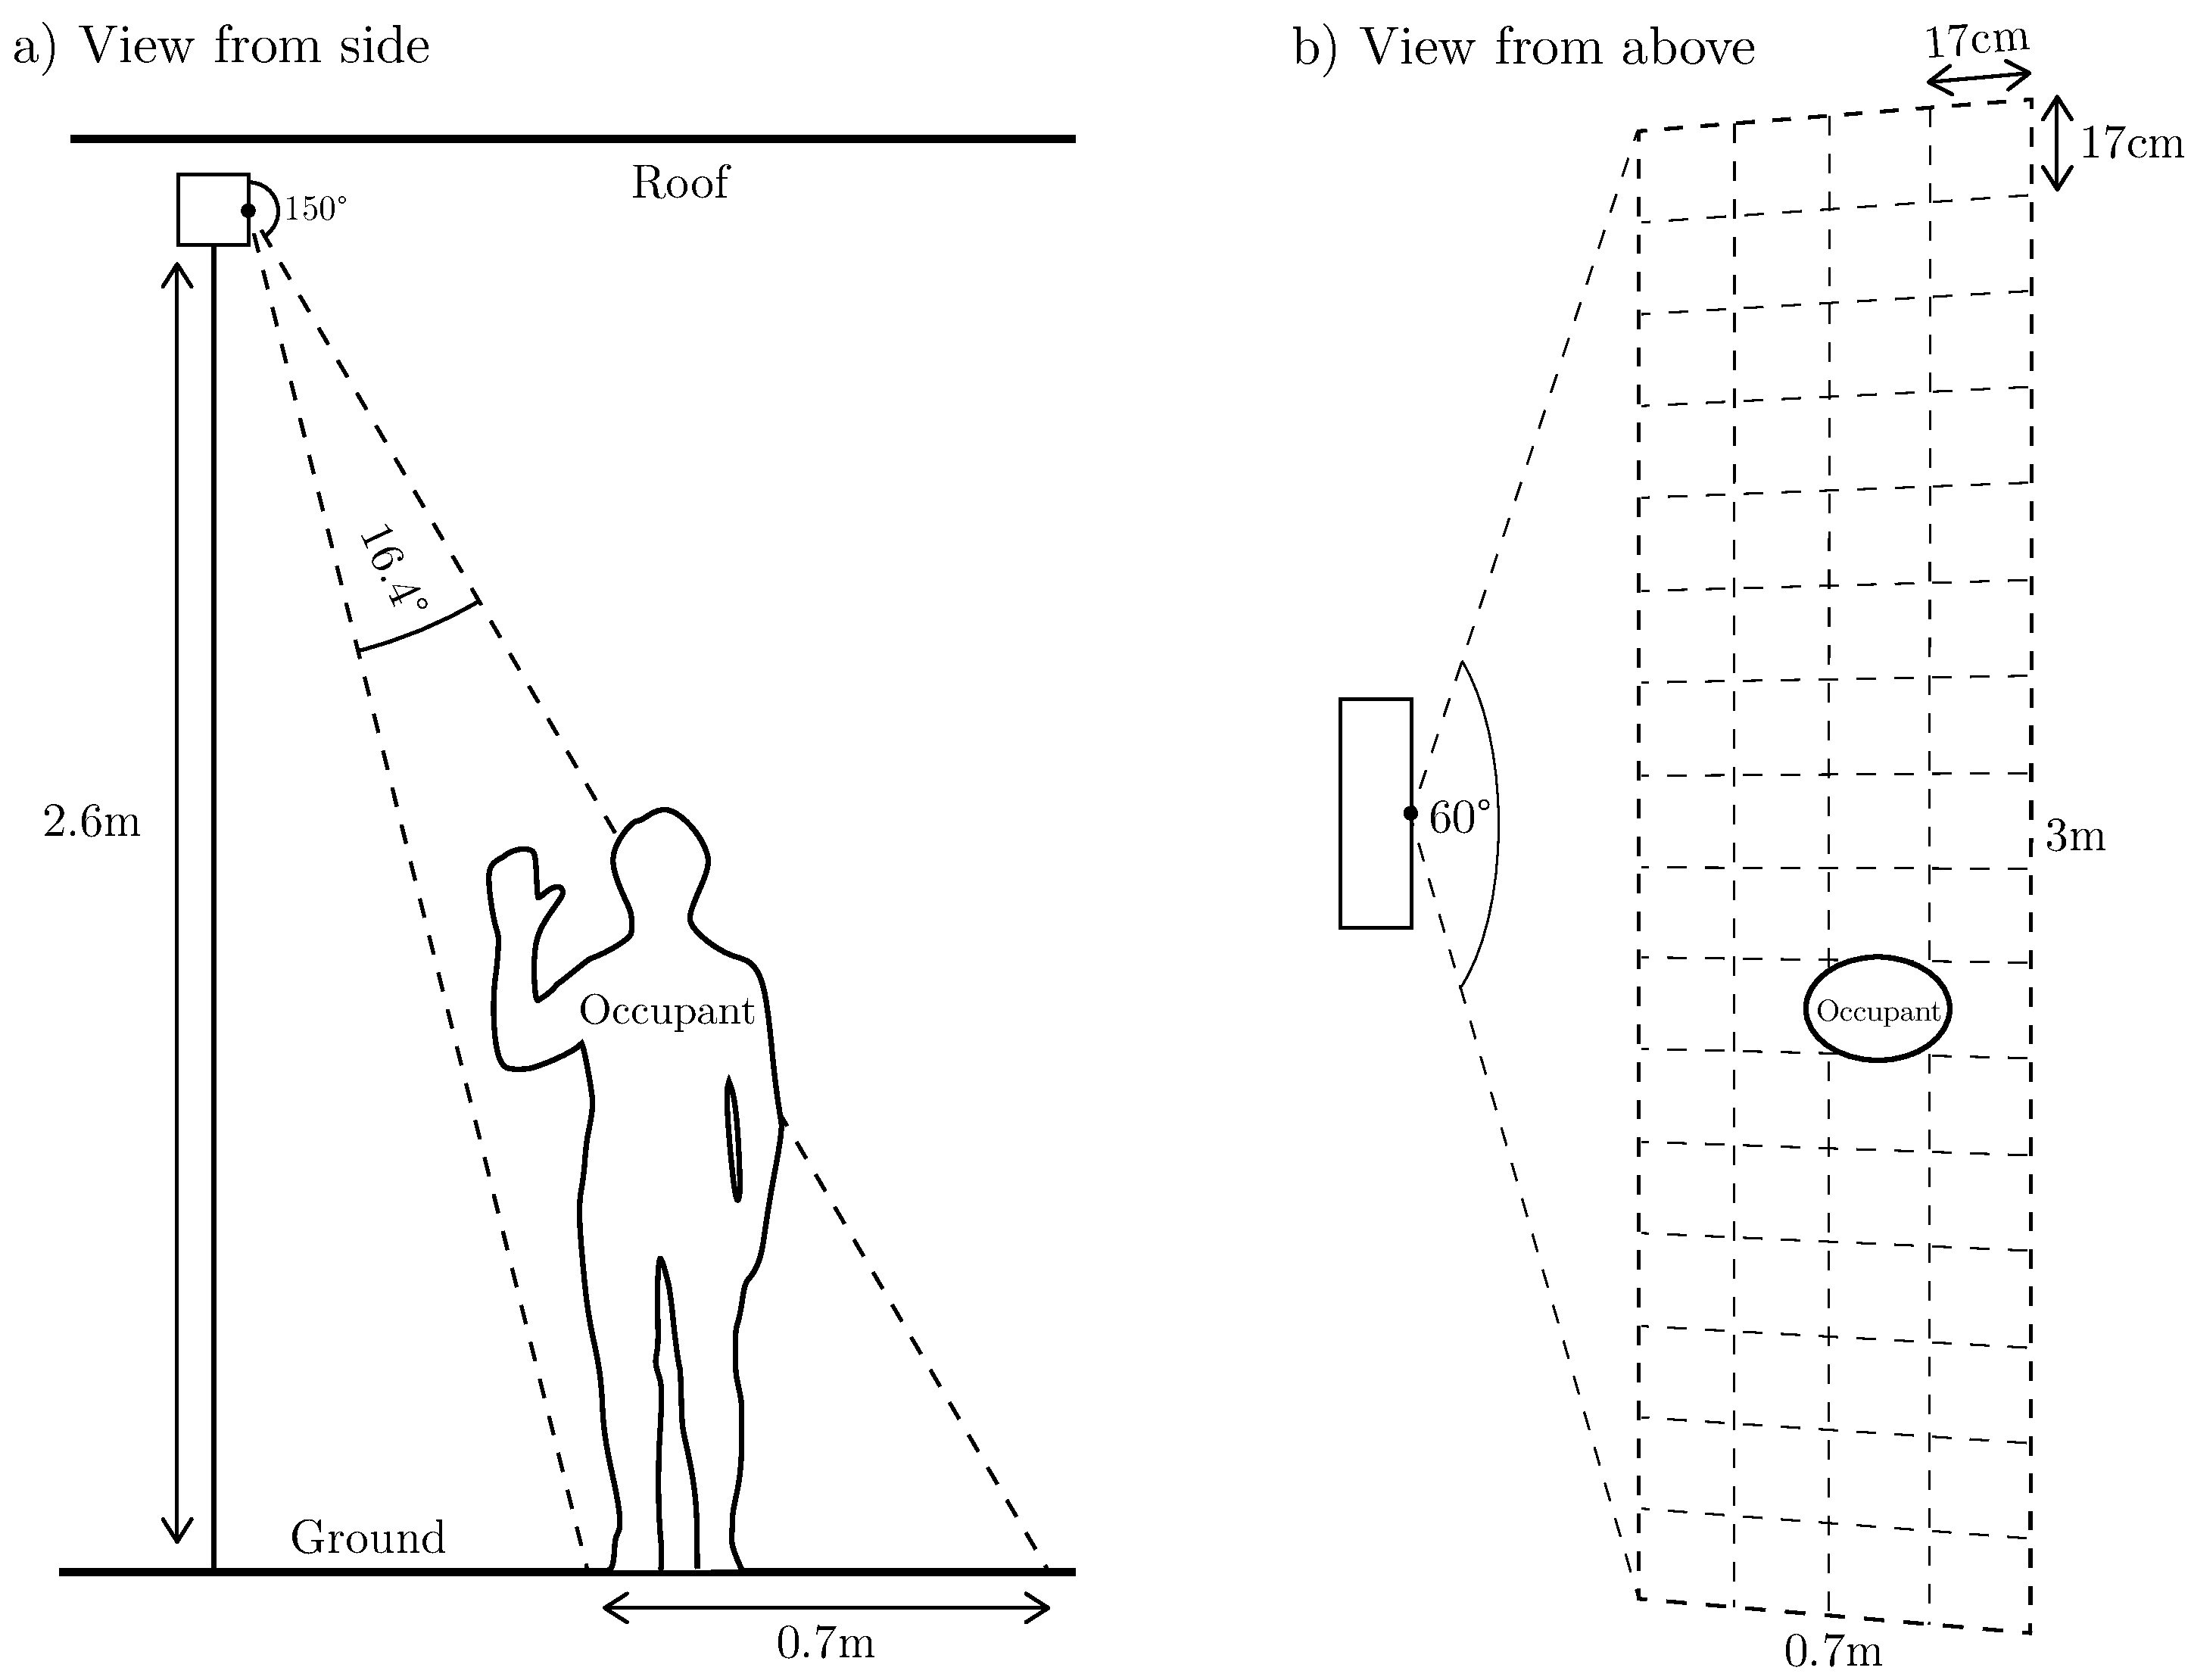
\includegraphics[height=\textheight]{../diagrams/third-exp-setup2.pdf}
 \caption{Classifier Experiment Set 1 Setup}
 \label{fig:exps:3setup}
 \end{figure}
\end{landscape}

 \ifcsdef{mainfile}{}{\bibliography{../references/primary}}
\end{document}
